Use the sweat data in Table 5.1 (See Example 5.2.) Find simultaneous 95\% $T^{2}$ confidence
intervals for $\mu_{1}$, $\mu_{2}$, and $\mu_{3}$ using Result 5.3. Construct the 95\% Bonferroni intervals
using (5--29). Compare the two sets of intervals.
\newline
\newline
Simultaneous 95\% $T^{2}$ confidence intervals:
\begin{align*}
    3.3978  &\leq \mu_{1} \leq  5.8822 \\
    35.0524 &\leq \mu_{2} \leq 55.7476 \\
    8.5707  &\leq \mu_{3} \leq 11.3593
\end{align*}

95\% Bonferroni confidence intervals
\begin{align*}
    3.6440  &\leq \mu_{1} \leq 5.6360 \\
    37.1031 &\leq \mu_{1} \leq 53.6969 \\
    8.8470  &\leq \mu_{1} \leq 11.0830
\end{align*}

As expected, the Bonferroni intervals are slightly more narrow than the simultaneous $T^{2}$ intervals.
Here's a visual representation of that with the 2D simultaneous $T^{2}$ ellipses and the projections onto the component axes. The dotted lines are the simultaneous $T^{2}$ intervals and the dashed lines are the Bonferroni intervals.

\begin{figure}[H]
    \centering
    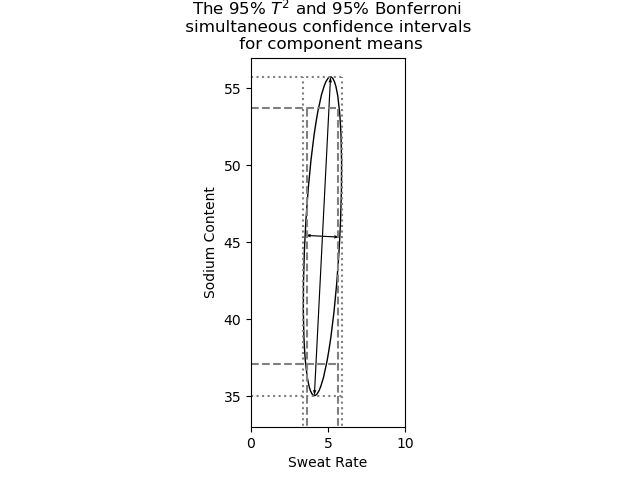
\includegraphics[scale=0.75]{./python/chapter-5/Question-5-7-CI-Sweat-Sodium.png}
\end{figure}

\begin{figure}[H]
    \centering
    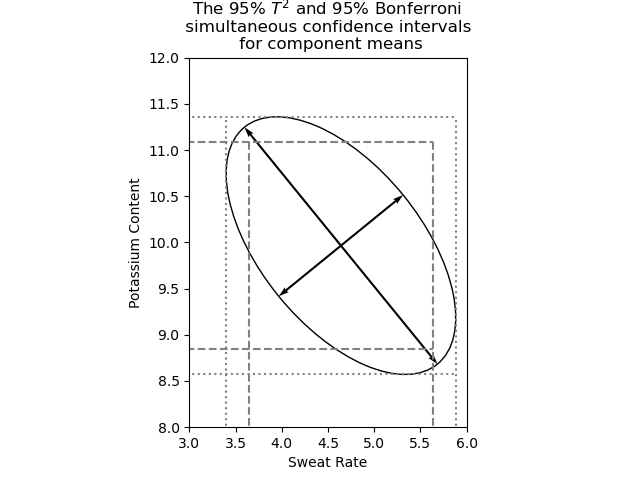
\includegraphics[scale=0.75]{./python/chapter-5/Question-5-7-CI-Sweat-Potassium.png}
\end{figure}

\begin{figure}[H]
    \centering
    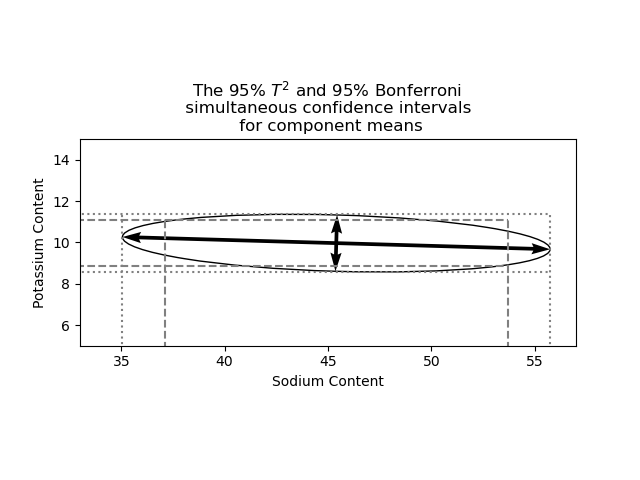
\includegraphics[scale=0.75]{./python/chapter-5/Question-5-7-CI-Sodium-Potassium.png}
\end{figure}

